%%
%% Copyright 2024 OXFORD UNIVERSITY PRESS
%%
%% This file is part of the 'mam-authoring-template Bundle'.
%% ---------------------------------------------
%%
%% It may be distributed under the conditions of the LaTeX Project Public
%% License, either version 1.2 of this license or (at your option) any
%% later version.  The latest version of this license is in
%%    http://www.latex-project.org/lppl.txt
%% and version 1.2 or later is part of all distributions of LaTeX
%% version 1999/12/01 or later.
%%
%% The list of all files belonging to the 'mam-authoring-template Bundle' is
%% given in the file `manifest.txt'.
%%
%% Template article for Microscopy and Microanalysis' document class `mam-authoring-template'
%% with bibliographic references
%%

\documentclass[unnumsec,webpdf,modern,large]{mam-authoring-template}%
\usepackage{amsmath,amssymb}
\usepackage{upgreek}
% natbib is already loaded by the document class
\bibliographystyle{plainnat}

% Suppress underfull hbox warnings
\hbadness=10000

\newcommand{\myfixed}{{\,\textrm{fixed}}}
\newcommand{\set}[1]{\left\{ #1 \right\}}
\newcommand{\myhier}{\textrm{hier}}
\newcommand{\myall}{\textrm{all}}
\newcommand{\mypair}{\textrm{pair}}
\newcommand{\myvar}{\textrm{var}}
\newcommand{\mygen}{\textrm{gen}}
\newcommand{\mysubsets}{\textrm{subsets}}
\newcommand{\mysource}{\textrm{source}}
\newcommand{\mysink}{\textrm{sink}}
\newcommand{\mytmp}{\textrm{tmp}}


%\usepackage{showframe}
\usepackage{upgreek}

\graphicspath{{figs/}}

% line numbers
%\usepackage[mathlines, switch]{lineno}
%\usepackage[right]{lineno}

\theoremstyle{thmstyleone}%
\newtheorem{theorem}{Theorem}%  meant for continuous numbers
%%\newtheorem{theorem}{Theorem}[section]% meant for sectionwise numbers
%% optional argument [theorem] produces theorem numbering sequence instead of independent numbers for Proposition
\newtheorem{proposition}[theorem]{Proposition}%
%%\newtheorem{proposition}{Proposition}% to get separate numbers for theorem and proposition etc.
\theoremstyle{thmstyletwo}%
\newtheorem{example}{Example}%
\newtheorem{remark}{Remark}%
\theoremstyle{thmstylethree}%
\newtheorem{definition}{Definition}

\begin{document}

\journaltitle{bioR$\upchi$i$\upnu$}
%\DOI{DOI HERE}
\copyrightyear{2025}
\pubyear{2025}
%\access{Advance Access Publication Date: Day Month Year}
\appnotes{Original Article}

\firstpage{1}

%\subtitle{Subject Section}

\title[PoolParty]{PoolParty: streamlined design of DNA sequence libraries in Python}

\author[1]{Zhihan Liu}
\author[1,$\ast$]{Justin B. Kinney\ORCID{0000-0003-1897-3778}}

\authormark{Liu and Kinney}

\address[1]{\orgdiv{Simons Center for Quantitative Biology}, \orgname{Cold Spring Harbor Laboratory}, \orgaddress{\street{1 Bungtown Rd.}, \postcode{11724}, \state{New York}, \country{United States}}}

\corresp[$\ast$]{Corresponding author. \href{email:jkinney@cshl.edu}{jkinney@cshl.edu}}

\received{Date}{0}{Year}
\revised{Date}{0}{Year}
\accepted{Date}{0}{Year}

\abstract{\textbf{Summary}: Computationally designed DNA sequence libraries (also called oligonucleotide pools) are widely used in massively parallel reporter assays (MPRAs), protein deep mutational scanning (DMS) experiments, and other multiplexed assays of variant effect (MAVEs). Increasingly, such libraries are also being used to analyze and interpret genomic AI models in silico. Despite their importance, the process of designing these libraries remains tedious and error-prone due to the lack of purpose-built software. Here we introduce PoolParty, a Python package that enables the streamlined design of sequence libraries using a declarative, composable syntax. In PoolParty, users build libraries by chaining together a core set of operations and sequence transformations, yielding a directed acyclic graph (DAG). This makes it possible to specify complex library designs (e.g., mixing multiple types of systematic and random variation across multiple sequence regions) in just a few lines of code. PoolParty automatically generates informative names for each sequence, as well as ``design cards'' that describe the specific set of operations used to generate the sequence. Over 20 built-in operation types cover nucleotide- and codon-level mutagenesis, motif insertion, deletion and insertion scans, barcode generation, and more. Visualization methods let users quickly audit library content and inspect the DAG. PoolParty thus transforms oligonucleotide pool design from ad hoc scripting into a structured, transparent, and reproducible process. \\
\textbf{Availability and implementation:} PoolParty can be installed using the pip package manager and is compatible with Python $\geq$ 3.10. Documentation is provided at http://poolparty.readthedocs.io; source code is available at http://github.com/jbkinney/poolparty.\\
\textbf{Contact:} jkinney@cshl.edu (J.B.K.)}


\maketitle

\section{Introduction}

Oligonucleotide pools have become essential tools in functional genomics. In massively parallel reporter assays (MPRAs), designed libraries of DNA sequences are routinely used to measure the regulatory activities of tens of thousands of candidate or variant regulatory elements in a single experiment \citep{Inoue2015cs}. In deep mutational scanning (DMS) experiments, coding sequences that have been either systematically or randomly mutagenized are commonly used to map protein fitness landscapes \citep{Fowler2014gq}. Both MPRAs and DMS experiments are examples of multiplexed assays of variant effect (MAVEs), a large and expanding family of high-throughput methods that quantitatively link sequence to function at scale \citep{Kinney2019jc}. The same idea extends beyond the wet lab: complex DNA sequence libraries are increasingly being used in silico to probe the behavior of genomic AI models \citep{Avsec2021bpnet, Nagai2026review}.

Computationally designing these libraries is straightforward in principle, but in practice it is tedious and error-prone. Typical applications require oligo pools that comprise multiple types of variant sequences generated in multiple ways. A DMS library, for example, might combine exhaustive single-amino-acid substitutions, sampled higher-order mutants, wild-type replicates, and barcodes — each generated by a different procedure and subject to different coverage requirements. An MPRA library might tile multiple transcription factor binding sites across a regulatory element in all possible orders and orientations, then assign each variant multiple barcodes. Coordinating this kind of combinatorial logic in a one-off script quickly becomes unwieldy, and subtle errors are hard to catch.

Existing tools can help with parts of the process, but none provide a unified framework for library design. General-purpose sequence toolkits \citep{Cock2009df, Schreiber2025nd, Pereira2015wj, Klie2023kg} can manipulate individual sequences but have no notion of a variant library as a structured object; in practice, users must write custom scripts to handle the combinatorial logic themselves. Assay-specific tools automate library design for particular experimental formats but are not easily adapted to novel designs \citep{GeorgakopoulosSoares2017gb, Ghazi2018aa, Barbon2022th}. And sequence optimization tools such as DnaChisel \citep{Zulkower2020jk} and CodonGenie \citep{Swainston2017rb} address synthesis constraints on individual sequences, not library-level design.

Here we present PoolParty, a Python package that enables the streamlined design of complex sequence libraries. In PoolParty, libraries are represented as objects called Pools, while individual steps in the sequence generation process are called Operations. Using a concise and transparent syntax, users chain together Operations into a directed acyclic graph (DAG) that yields the desired Pool. The DAG describes the high-level logic used to generate sequences, while the procedural logic and bookkeeping are handled internally. Importantly, no sequences are generated until the user requests them, and only the requested sequences are generated. This makes it possible for users to explore and test multiple design options without triggering expensive computation. When sequences are generated, each is automatically assigned an informative name and paired with a \emph{design card} that records the specific procedures used to construct it. We demonstrate PoolParty in three example applications: a DMS library for protein GB1 modeled after \cite{Olson2014iq}, an MPRA library probing transcription factor binding site grammar, and an in silico experiment characterizing the behavior of SpliceAI \citep{Jaganathan2019ps} in which the design cards form the basis for surrogate modeling.

\section{Methods}

\subsection{Pools and Operations}

PoolParty is built around two core concepts: Pools and Operations. Pools represent collections of sequences---either the final library that the user wishes to generate, or intermediate sets of sequences out of which the final library is constructed. Operations represent the steps used to create Pools. When designing a library, users chain together multiple Operations into a DAG that yields the desired Pool. Sequences are then generated on demand from the final Pool (the \emph{root Pool}) using the DAG. By delaying sequence generation until it is explicitly requested, users can test many different library designs --- inspecting a few sampled sequences from each --- before committing to generating the full library.  

PoolParty provides over 20 built-in Operations that users can choose from when constructing DAGs. Each Operation takes zero or more Pools as input and returns exactly one Pool as output. It is useful to think of Operations as falling into four functional categories (Fig.~\ref{fig:figure1}A): Source Operations, Transformation Operations, Composition Operations, and State Operations. \emph{Source Operations} create the initial Pools from which all downstream Pools are constructed. These many represent user-specified sequences, DNA sequences generated using position weight matrices or IUPAC motifs, random k-mers, barcodes, and so on. \emph{Transformation Operations} modify sequence content, e.g., generating sequence variants through point mutations, insertions, deletions, recombination, or shuffling. Specialized codon-aware Operations are provided for transformations that operate on open reading frames. \emph{Composition Operations} combine sequences from multiple parent Pools, either by concatenating parent sequences end-to-end (the \texttt{join} Operation) or by merging multiple Pools into one Pool (the \texttt{stack} Operation). \emph{State Operations} affect which sequences are in a Pool and how they are ordered, and include methods to select, reorder, filter, and replicate sequences.

\subsection{Sequence generation}

To generate a sequence, PoolParty passes a \emph{state} --- an integer index that, together with a random seed, uniquely determines the output --- to the root Pool. Generation then proceeds in two passes (Fig.~1B). In the \emph{backward pass}, PoolParty propagates the state from the root Pool back through the DAG. Each Operation decomposes the state it receives into an internal state and one or more states that are then passed to its input Pools. Each of the input Pools then passes its assigned state to its upstream Operation. In the \emph{forward pass}, each Operation generates a sequence based on its input sequences (if any) and its internal state. This process starts at the source Operations and proceeds forward until the root Pool receives the completed sequence. To generate a full library, PoolParty iterates the state passed to the root Pool from zero up to the desired library size.

\subsection{Operation modes}

Each Operation has a mode that determines how it interprets its internal state. Operations can run in one of three modes:

\begin{itemize}
\item In \textbf{sequential mode}, the Operation exhaustively enumerates a finite set of design choices. For example, \texttt{mutagenize} in sequential mode with single-nucleotide mutations yields one variant for every possible mutation at every target position. The internal state indexes which specific mutation is applied.

\item In \textbf{random mode}, design choices are sampled stochastically. For example, the \texttt{shuffle} Operation randomly reorders the bases in a sequence. Users can optionally fix the number of samples, producing a reproducible set of variants. A master seed ensures reproducibility.

\item In \textbf{fixed mode}, the output is uniquely determined by the input sequences. For example, \texttt{join} concatenates its input sequences without modification.
\end{itemize}

\subsection{StateTracker}

Each Operation's backward-pass decomposition is designed to reverse its forward-pass composition. For most Operations, the output state is the Cartesian product of the Operation's internal state and its input Pool states, so the backward pass uses mixed-radix decomposition to recover the constituents. The \texttt{stack} Operation is different: its output states are the disjoint union of its input Pool states, so each output state maps to exactly one parent. Keeping track of these composition rules across a complex DAG is error-prone, so we developed a back-end package called StateTracker that automates state composition and decomposition throughout the graph. During library specification, StateTracker resolves the state structure of every Pool from the DAG alone, and the state count of the root Pool defines the default library size. No sequences are generated at this stage.

\subsection{Sequence regions}

One often wants to perform different operations on different parts of a template sequence. To facilitate this, PoolParty lets users mark regions of interest within sequences using XML-style tags. Content tags enclose an existing sub-sequence (e.g., \texttt{AAA<cre>CCCGGG</cre>TTT}), while self-closing tags mark insertion points (e.g., \texttt{ACGT<ins/>ACGT}). Operations can then be instructed to act only on a named region, as illustrated in Fig.~\ref{fig:figure1}C. Tags persist through the DAG and remain valid even when upstream Operations change the content or length within a region, so multiple Operations can reliably target the same region in series.

\subsection{Sequence metadata}

When generating a library, it is often useful to record how each sequence was constructed. PoolParty provides three complementary features that enable this, each of which is illustrated in Fig.~\ref{fig:figure1}C and described below.

\begin{itemize}
\item \textbf{Design cards} record the design choices used to generate each sequence. Users specify which Operations and Operation-specific parameters to track. The resulting cards are then returned as a DataFrame alongside the generated sequences. Each row corresponds to one sequence, and its columns record the values of the tracked operation parameters. As structured metadata, design cards support downstream filtering, grouping, and modeling without custom sequence parsing.

\item \textbf{Sequence names} summarize the construction history of each sequence in an easily readable format. Users assign a prefix to each Operation they wish to track. PoolParty then combines each prefix with the corresponding resolved state to form the name. For example, \texttt{wt.mut\_03.bc\_01} denotes a wild-type sequence with mutation variant~3 and barcode~1.

\item \textbf{Sequence styling} visually annotates sequences with colors and text formatting that reflect their construction history. For example, \texttt{mutagenize} can be instructed to mark the positions it mutates in bold yellow text, making these positions stand out from the rest of the sequence. This formatting uses ANSI escape codes, so output renders correctly in terminals, Jupyter notebooks, and other environments that support formatted text. Importantly, styles combine in a natural manner as sequences propagate through the DAG, e.g., a mutated base can appear highlighted in red within an inserted motif shown in blue.
\end{itemize}

%TODO: In panel C, replace "S=" and "S'=" with "num_states=". 
\begin{figure*}[t]
\centering
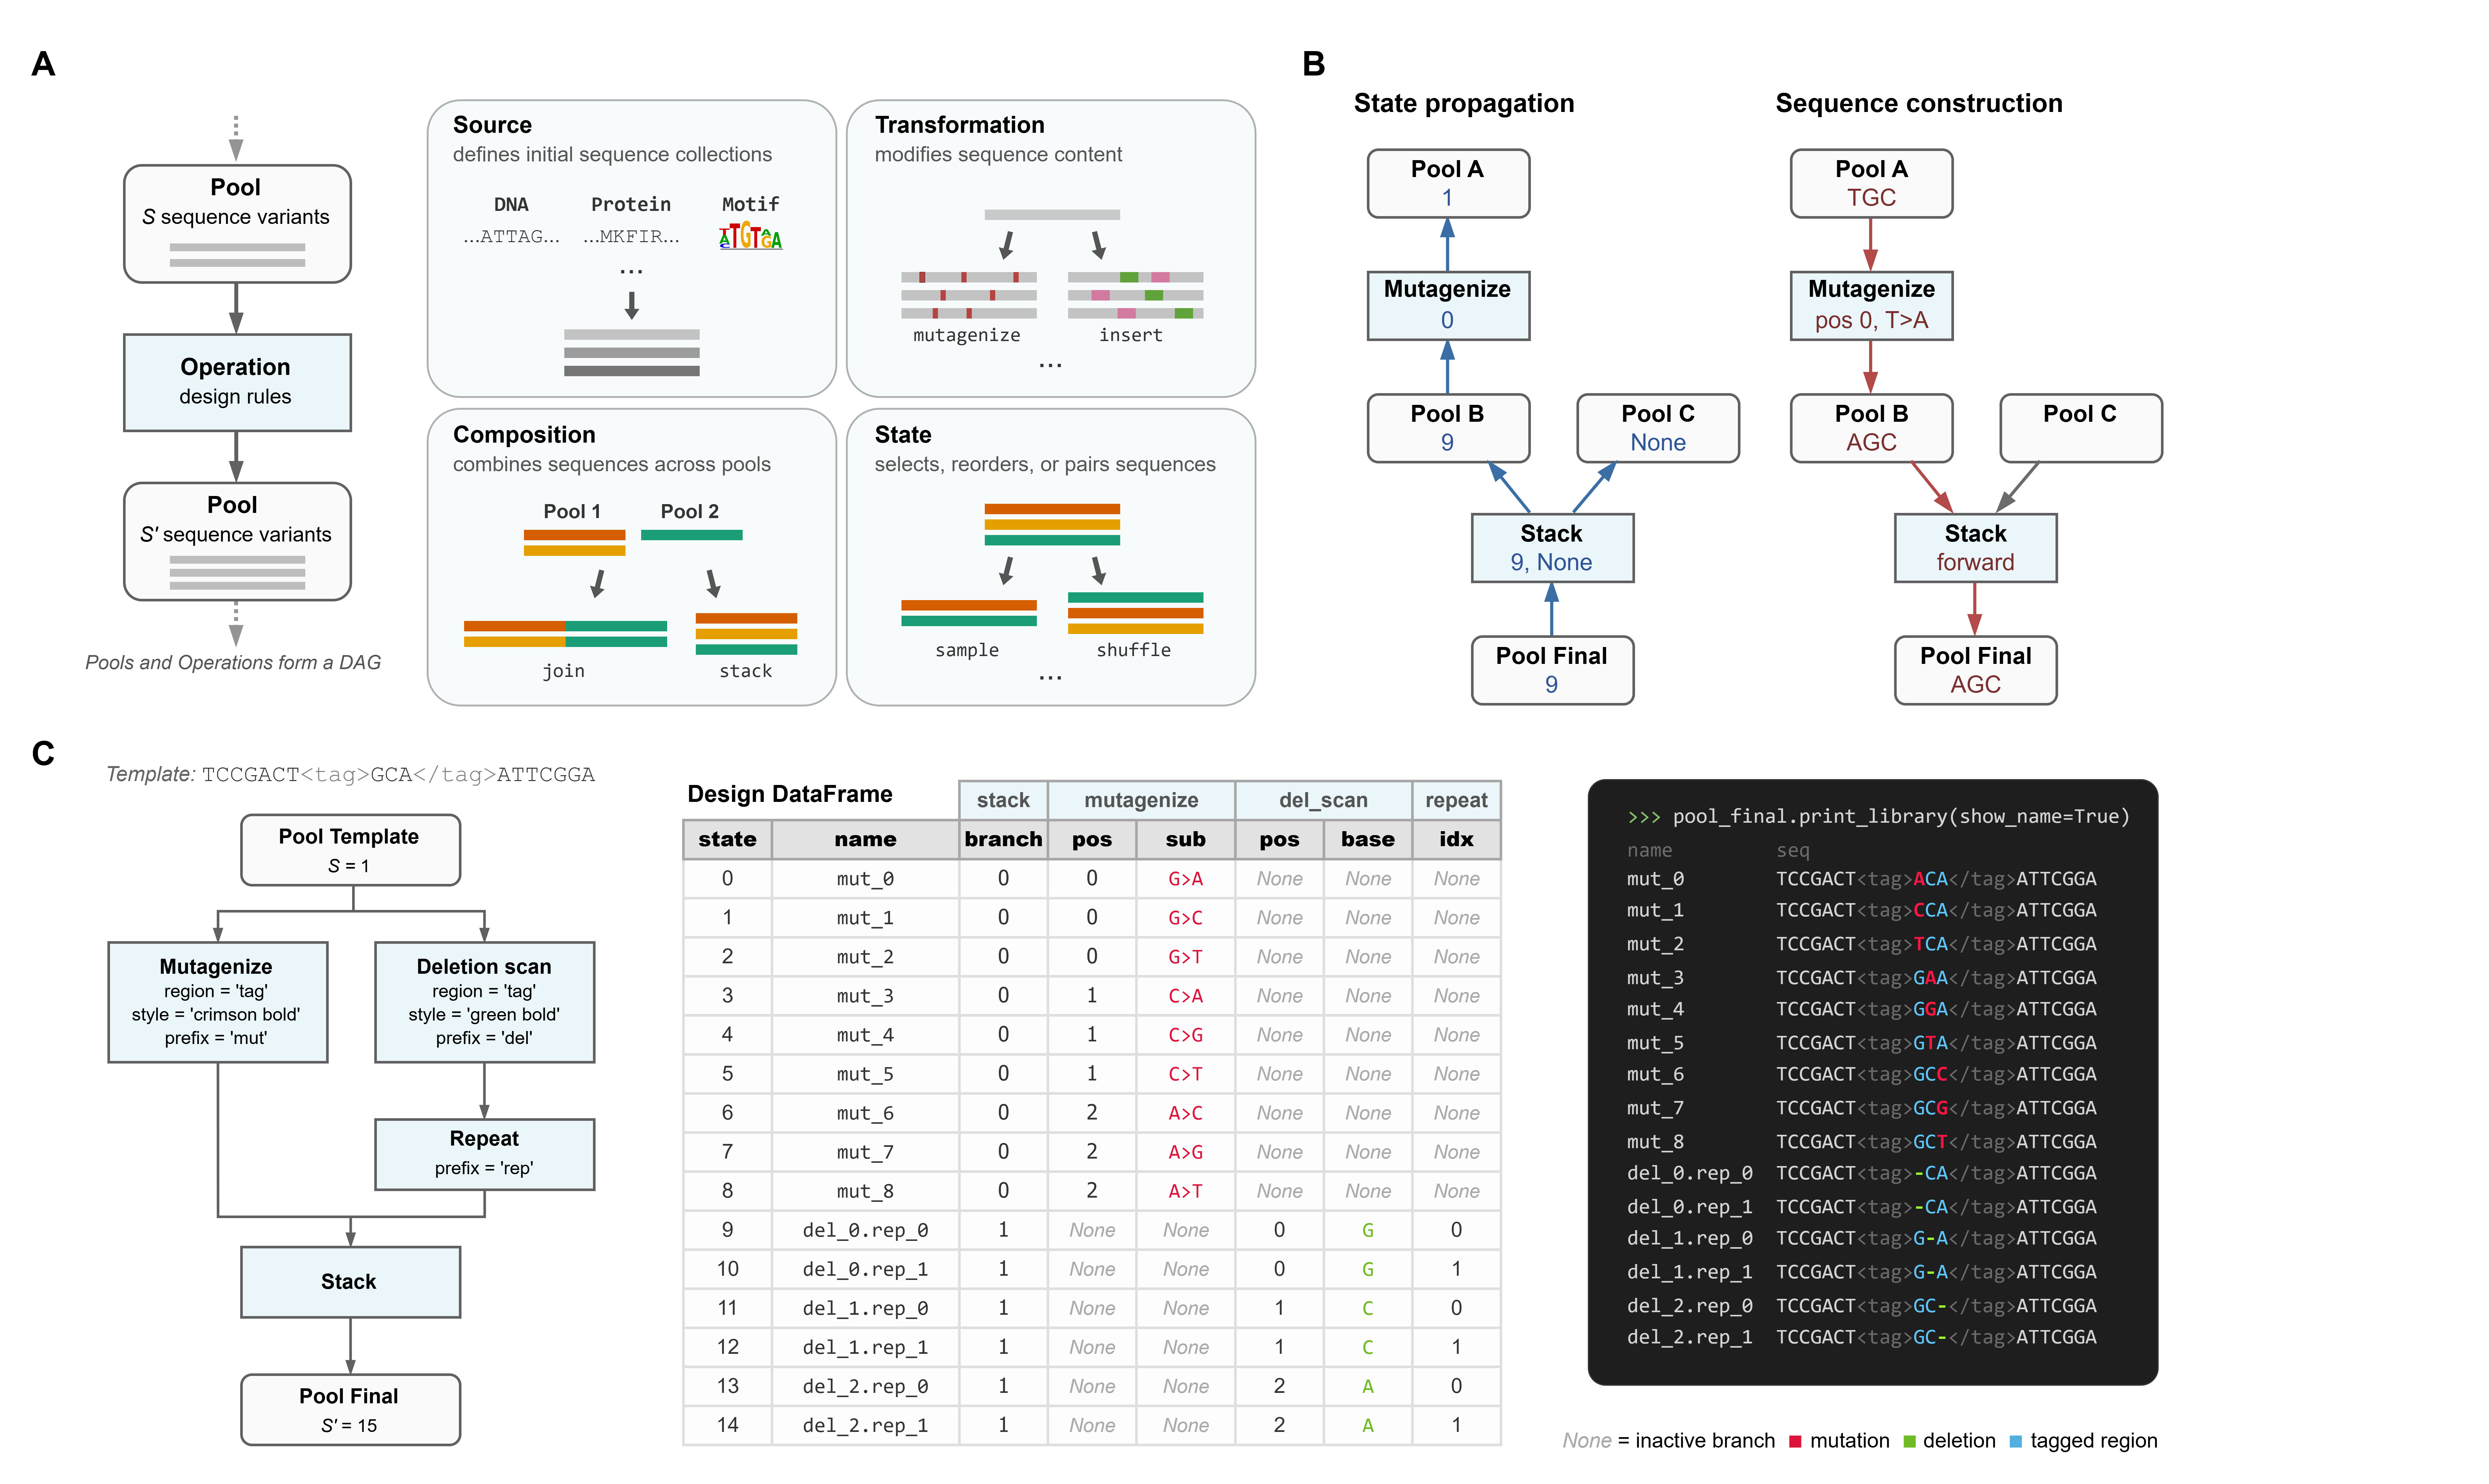
\includegraphics[width=\textwidth]{figure1_v2.png}
\caption{\textbf{PoolParty builds libraries from Pools and Operations.}
\textbf{(A)} Pools represent collections of sequences and Operations generate new Pools based on their inputs (left). Users chain Operations into a directed acyclic graph (DAG) that specifies the desired library, but delays sequence generation until the user requests it. Operations fall into four functional categories: source, transformation, composition, and state (right).
\textbf{(B)} Sequence generation proceeds in two passes. For each desired sequence, PoolParty passes a number (called the \emph{state}) that specifies which sequence to generate to the root Pool. This state is propagated backward through the DAG, resolving the internal state of every Operation along the way (left). A subsequent forward pass then causes each Operation to generate and combine sequence fragments according to its resolved state, producing the final sequence at the root Pool (right). When multiple Pools are combined by \texttt{stack}, only one parent is active for a given state; inactive branches receive no state (\texttt{None}) and are shown as grey arrows.
\textbf{(C)} Example workflow. The template sequence contains a user-specified region (called ``tag'') that is targeted for both mutagenesis and deletion scanning. Left: the DAG specifying the sequence library. Center: the design card DataFrame returned by the DAG. Right: styled sequence output, with colors indicating mutations (red), deletions (green), and the tagged region (blue).}
\label{fig:figure1}
\end{figure*}

\subsection{Implementation and extensibility}

PoolParty requires Python 3.10 or later, is designed to have minimal dependencies, and is distributed via PyPI. Documentation, tutorials, and example notebooks are available on the ReadTheDocs and GitHub project websites. PoolParty is designed to be extensible: new Operation types can be created by subclassing the Operation base class and implementing a few required methods. Custom Operations automatically inherit support for state tracking, design card generation, and visualization, allowing researchers to add domain-specific operations without reimplementing core infrastructure.

\subsection{SpliceAI surrogate analysis}

This section provides technical details for the surrogate modeling analysis presented in Results. We sampled 9-mers from the human 5$'$ splice-site (5$'$ss) position weight matrix \citep{Wong2018quantitative} and scored them with MaxEntScan \citep{Yeo2004me}. Sequences were binned into 100 MaxEntScan score (hereafter, strength) quantiles, and 20 sequences were drawn from each bin (2,000 total). Each 9-mer was inserted at 100 positions flanking the SMN2 exon~7 canonical donor and paired with a matched control in which the GT dinucleotide was disrupted (T$>$A at $+2$; Fig.~4A).

We predicted SpliceAI donor probabilities at the canonical site using the five-model ensemble of \citet{Jaganathan2019ps} with $\pm$5~kb of genomic context (GRCh38). For each library-control pair, we computed the difference in logit-transformed predictions at the canonical donor. These per-sequence values were averaged within each cell of the resulting $100 \times 100$ position $\times$ strength grid (Fig.~4B).

We fit generalized additive models (GAMs) to the cell means using pyGAM \citep{Serven2018pg}, with smooth terms for position, strength, and their interaction. Models were weighted by the inverse variance of each cell mean. Exonic and intronic regions were modeled separately. Model performance was evaluated by checkerboard cross-validation of the grid.

\section{Example Applications}

\subsection{DMS library for protein GB1}

\begin{figure*}[t]
\centering
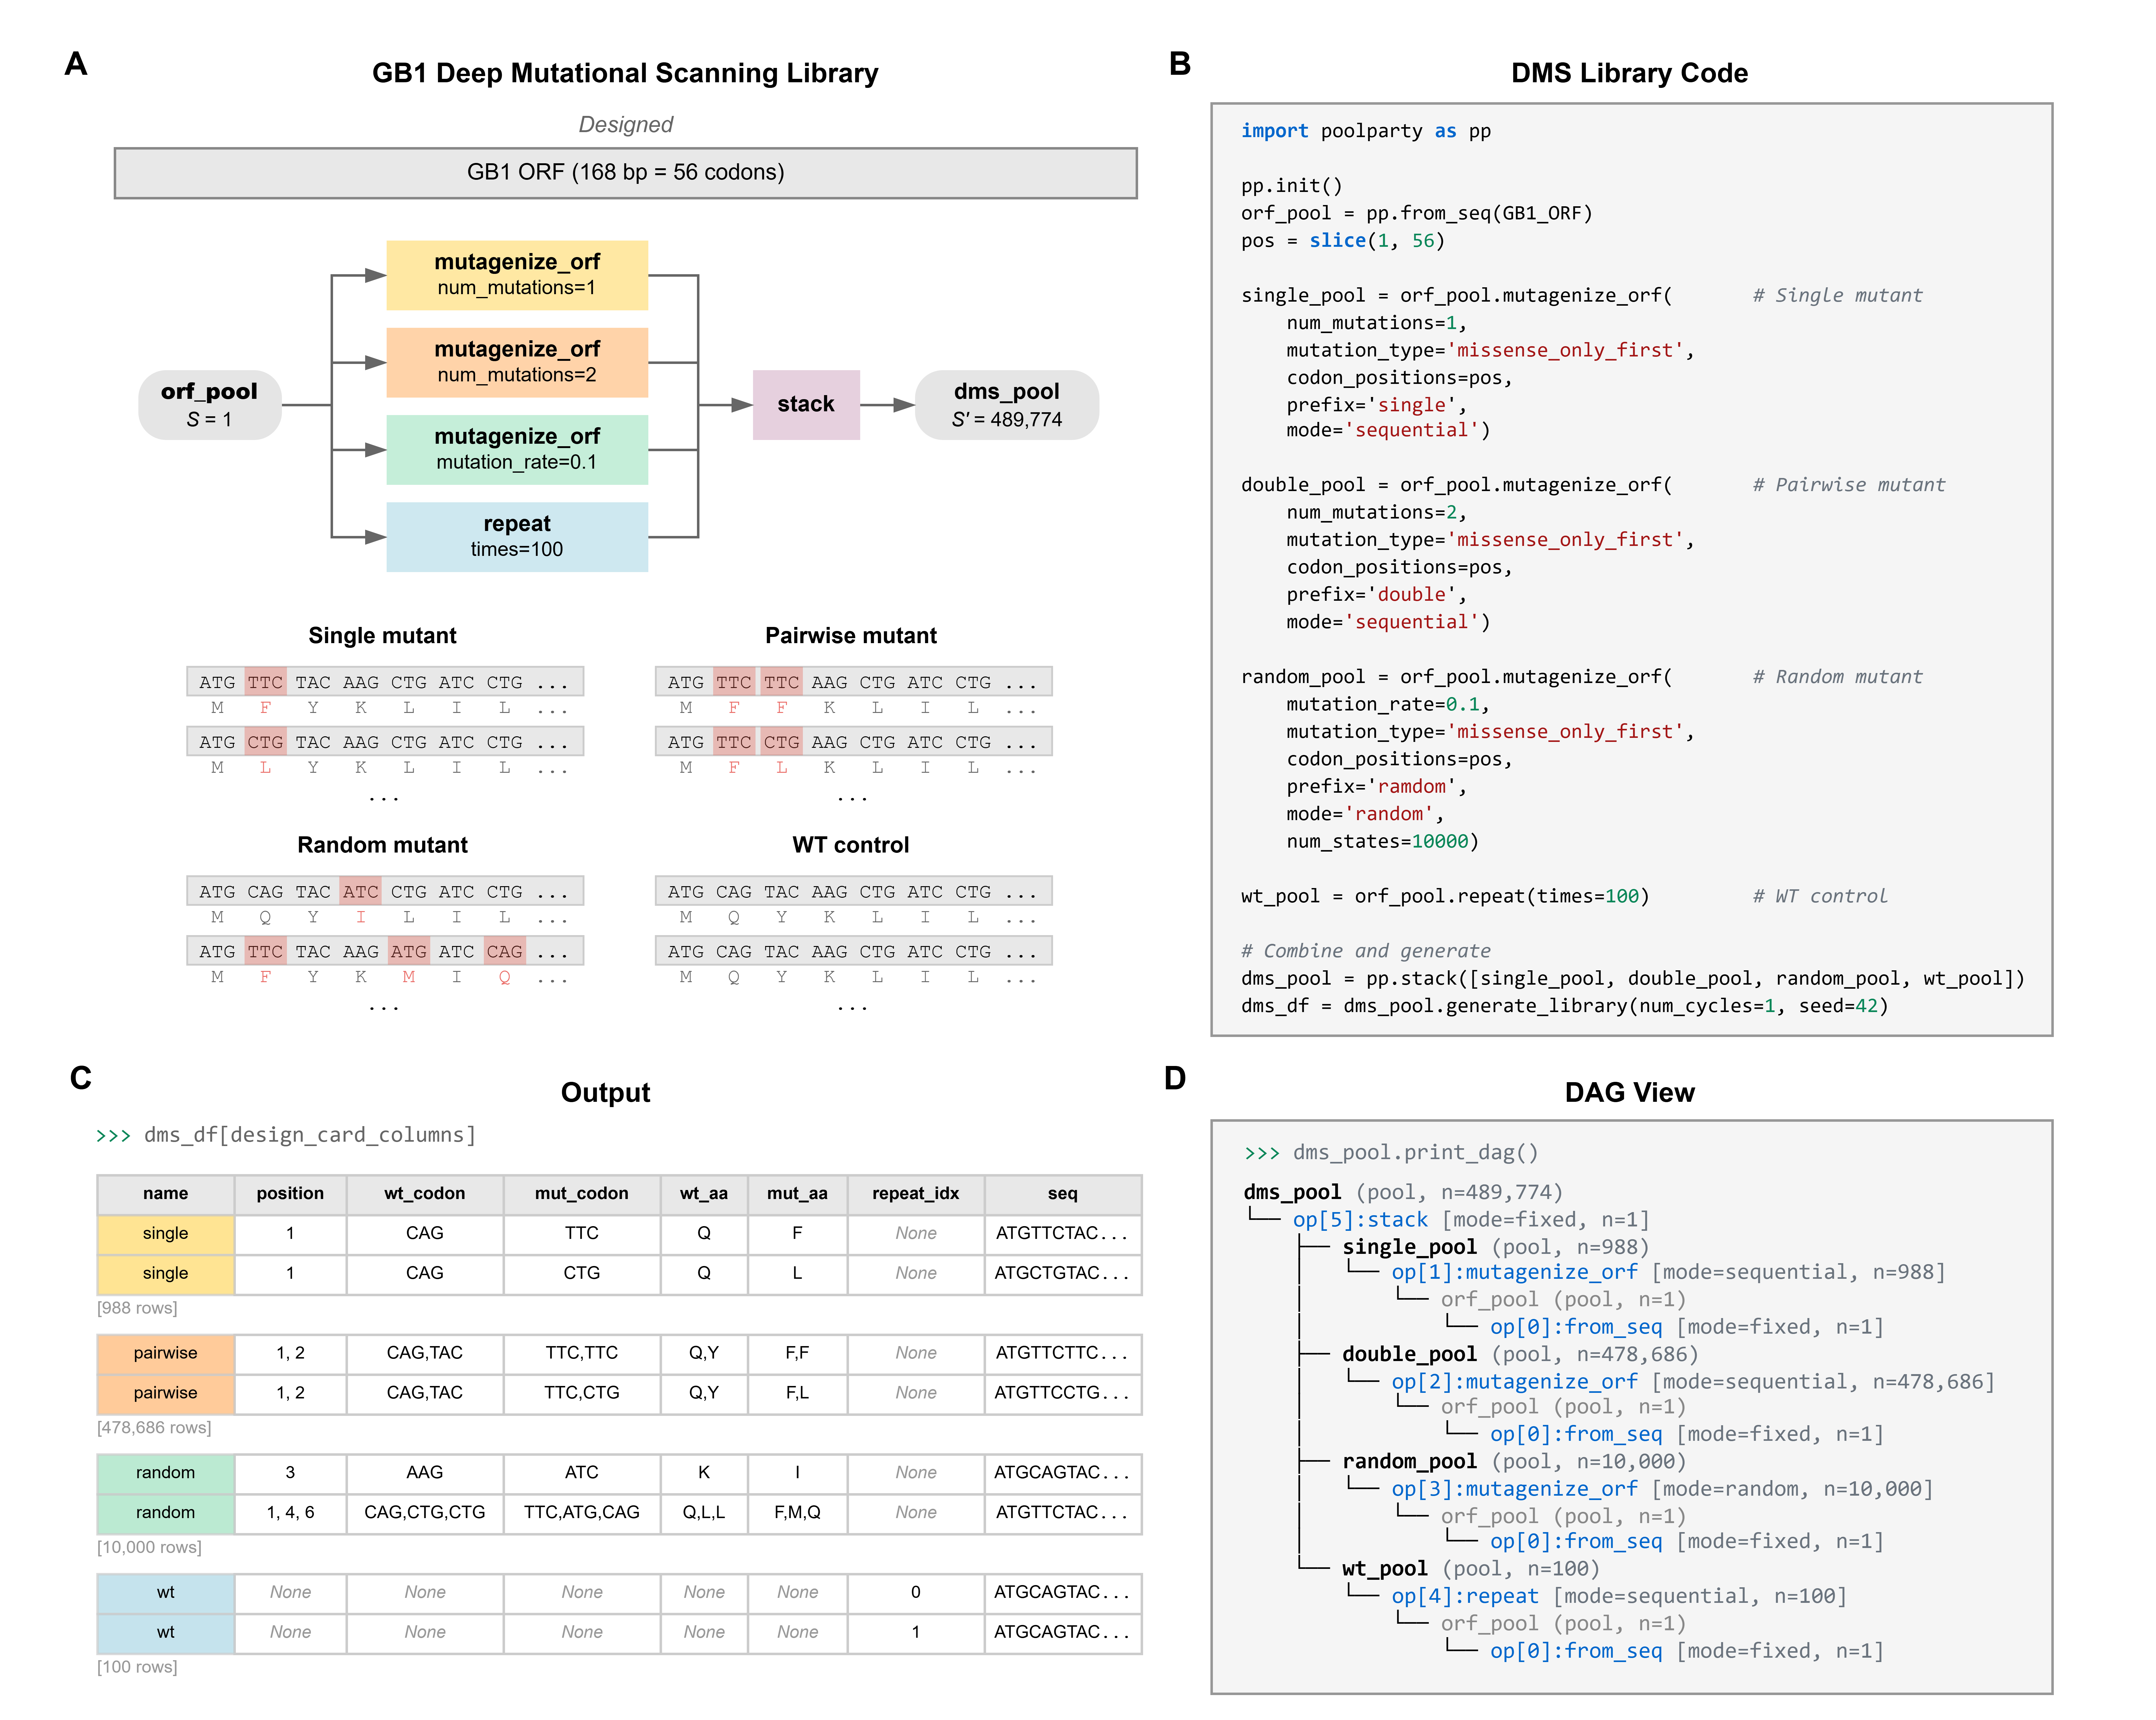
\includegraphics[width=\textwidth]{figure2_v2.png}
\caption{\textbf{PoolParty design of a GB1 deep mutational scanning library.}
\textbf{(A)} DAG and representative sequences for each of the four library components: single and pairwise amino acid substitutions, random higher-order mutants, and wild-type replicates. Mutated codons are highlighted with amino acid translations shown beneath.
\textbf{(B)} Python code implementing the DAG.
\textbf{(C)} Design cards reporting the library component, mutation positions, and amino acid changes for representative variants.
\textbf{(D)} DAG structure displayed by \texttt{print\_dag()}.}
\label{fig:figure2}
\end{figure*}

As a first example, we use PoolParty to reconstruct and extend the library used in a DMS experiment on protein GB1 by \citet{Olson2014iq}. Their library contained the wild-type GB1 coding sequence, all single amino acid mutations (excluding the start codon), and nearly all possible pairs of amino acid mutations. This library is substantially larger than most DMS libraries, containing over half a million variants. Its inclusion of so many pairwise variants has helped it become a benchmark dataset in the quantitative modeling of protein sequence-function relationships \citep{Otwinowski2018jb, Otwinowski2018jj, Tareen2022dh, Faure2024mn}.

Fig.\ \ref{fig:figure2}A illustrates the DAG used to construct this library; the code that establishes the DAG is shown in Fig.\ \ref{fig:figure2}B. First we define a Pool, named \texttt{orf\_pool}, that represents the wild-type GB1 coding sequence. This Pool is then fed as input to four separate branches. The first two branches use the \texttt{mutagenize\_orf} Operation in sequential mode to enumerate all 1,045 single and all 546,085 pairwise amino acid substitutions. A third branch uses \texttt{mutagenize\_orf} in random mode to generate 10,000 variants with mutations at 10\% of amino acid positions. Because \texttt{mutagenize\_orf} operates at the codon level, users specify only the desired amino acid substitutions, and PoolParty resolves the corresponding nucleotide changes. A fourth branch uses the \texttt{repeat} Operation to produce 100 wild-type replicates. All four branches are then merged by \texttt{stack} into a final library comprising 557,230 sequences. The design card provided with each variant (Fig.~\ref{fig:figure2}C) reports the component it derives from, the mutations it contains, and the replicate index (for wild-type sequences). Users can inspect the structure of the DAG by using the \texttt{print\_dag} method (Fig.~\ref{fig:figure2}D).


%%%%%%%%%%%%%%%%%%%%%%%%%%%%%%%%%%%%%%%%%%%%%%%%%%%%%%%%%%%
%%% Below is from manuscript_overleaf_26.03.17/main.tex %%%
%%%%%%%%%%%%%%%%%%%%%%%%%%%%%%%%%%%%%%%%%%%%%%%%%%%%%%%%%%%

\subsection{MPRA library design for regulatory grammar}

\begin{figure*}[t]
\centering
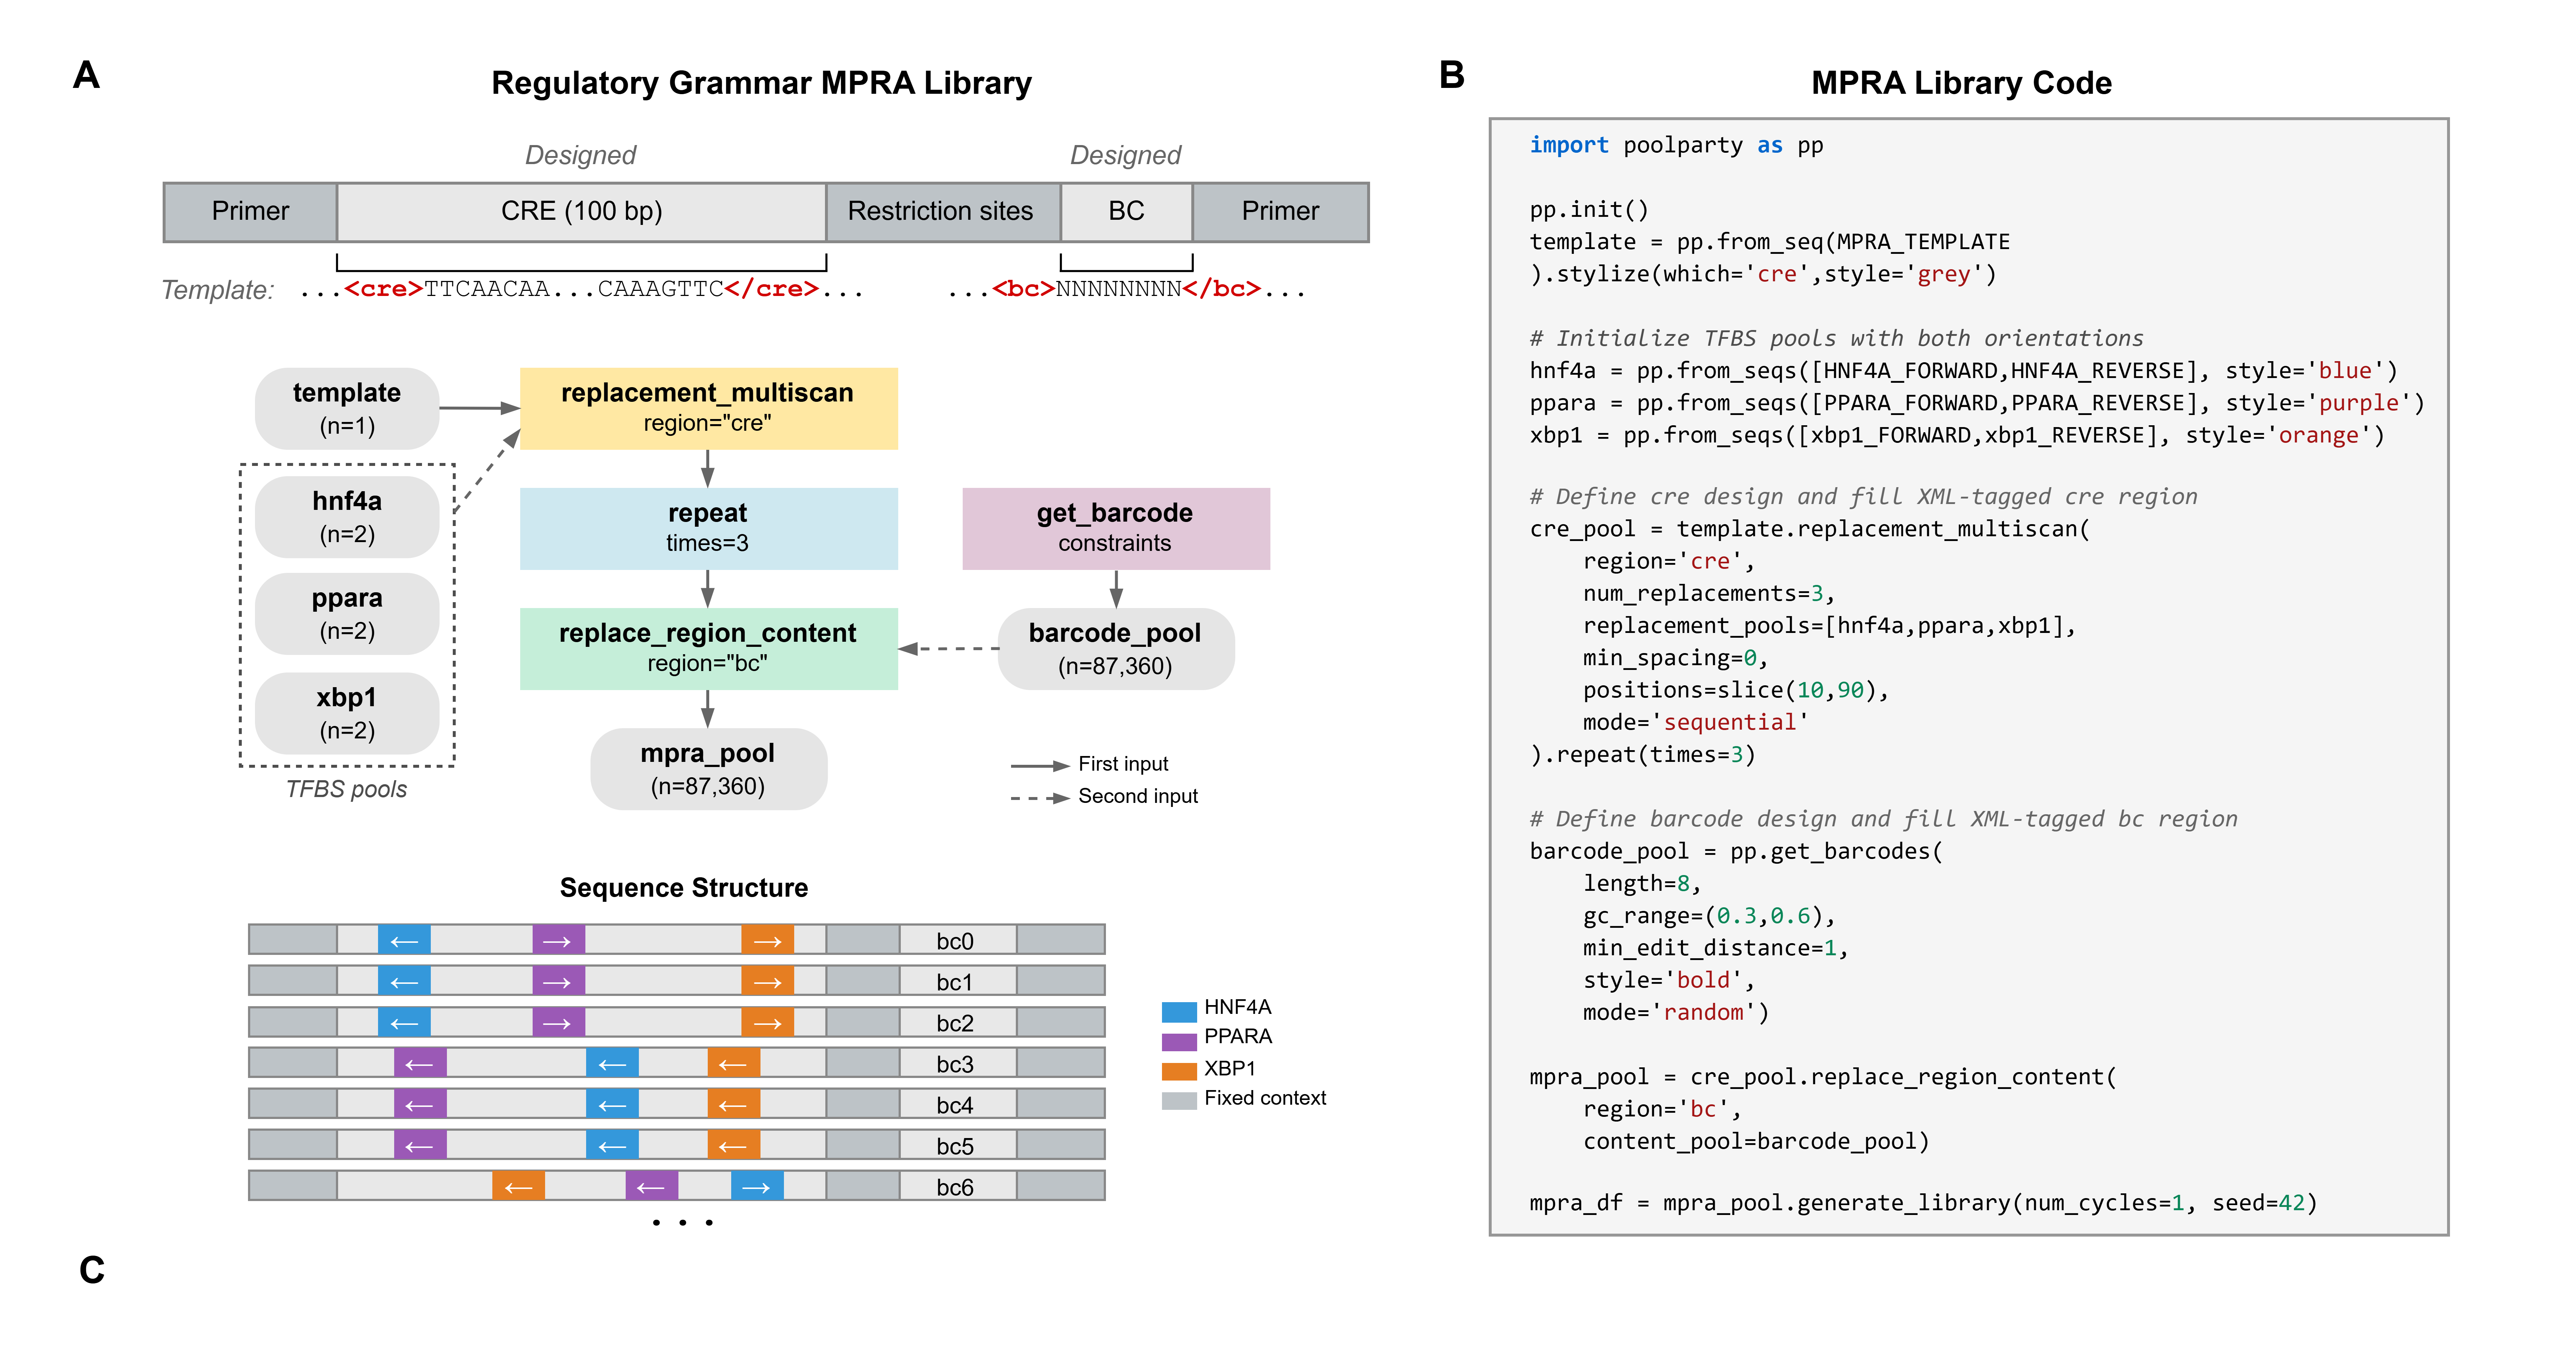
\includegraphics[width=\textwidth]{figure3_v2.png}
\caption{\textbf{Design of a regulatory grammar MPRA library using PoolParty.}
\textbf{(A)} Schematic of the regulatory grammar MPRA library targeting a 100-bp CRE. HNF4A, PPARA, and XBP1 binding sites are tiled across the CRE in different orders and orientations, with each variant assigned three unique barcodes (87,360 sequences total). Representative sequence structures are shown, with TFBS placements and barcode assignments indicated.
\textbf{(B)} Python code for library construction. TFBS pools are initialized with both forward and reverse-complement sequences to represent orientation.
\textbf{(C)} Example design cards. Representative rows are shown for each CRE variant, with insertion position, orientation, and barcode index recorded.}
\label{fig:figure3}
\end{figure*}

MPRAs use synthetic DNA sequences to dissect the cis-regulatory codes underlying a variety of gene regulatory steps. Unlike DMS experiments, MPRAs for regulatory grammar often involve systematically changing the spacing, order, orientation, and multiplicity of known regulatory motifs within an otherwise inert sequence. The combinatorial variation of these design parameters reveals how regulatory proteins bound at cognate sites orchestrate regulatory activity. For example, \citet{GeorgakopoulosSoares2023tf} tested over 200{,}000 sequences with all pairwise and triplet arrangements of 18 TFBSs in synthetic enhancers, and found that orientation and order are major drivers of expression. The scale and controlled design of these data also make them highly suited for training and benchmarking machine learning models \citep{Fleur2024decoding}.

As a second use case, we designed an MPRA library studying how binding site arrangements of three liver-enriched TFs affect regulatory activity (Fig.~3A,B). Following the oligo layout of \citet{Melnikov2012dw}, we define the template Pool from a sequence containing an inert 100~bp CRE region and a barcode region, both tagged with region markers (Section~2.3). Each of the three TFs --- HNF4A, PPARA, and XBP1 --- is represented by a Pool containing both the forward and reverse-complement binding sites. We use \texttt{replacement\_multiscan} in sequential mode to tile these Pools within the central 80~bp of the CRE without overlap. PoolParty automatically enumerates 2{,}184 valid placements, each in eight orientation combinations, for a CRE Pool of 17{,}472 variants. After repeating this Pool three times, we fill the barcode region with random barcodes from \texttt{get\_barcodes}, giving the final \texttt{mpra\_pool} of 87{,}360 sequences at a 1:3 CRE-to-barcode ratio (Fig.~3A). 

PoolParty supports two types of styling. The style parameter of Operations marks the modifications they introduce to the sequence, while the \texttt{stylize} Operation annotates a region of the existing sequence. We first use \texttt{stylize} to add a background color to the tagged CRE region in the template. For the inserts, we color each TFBS Pool using the style parameter in \texttt{from\_seqs} (HNF4A blue, PPARA purple, XBP1 orange) and mark barcodes bold in \texttt{get\_barcodes} (Fig.~3B). When the TFBSs are tiled into the CRE, their colors overlay the CRE region background color, and both are rendered in the \texttt{print\_library} output (Fig.~3C), making the positions and ordering of the three TFBSs immediately visible.


\begin{figure*}[p]
\centering
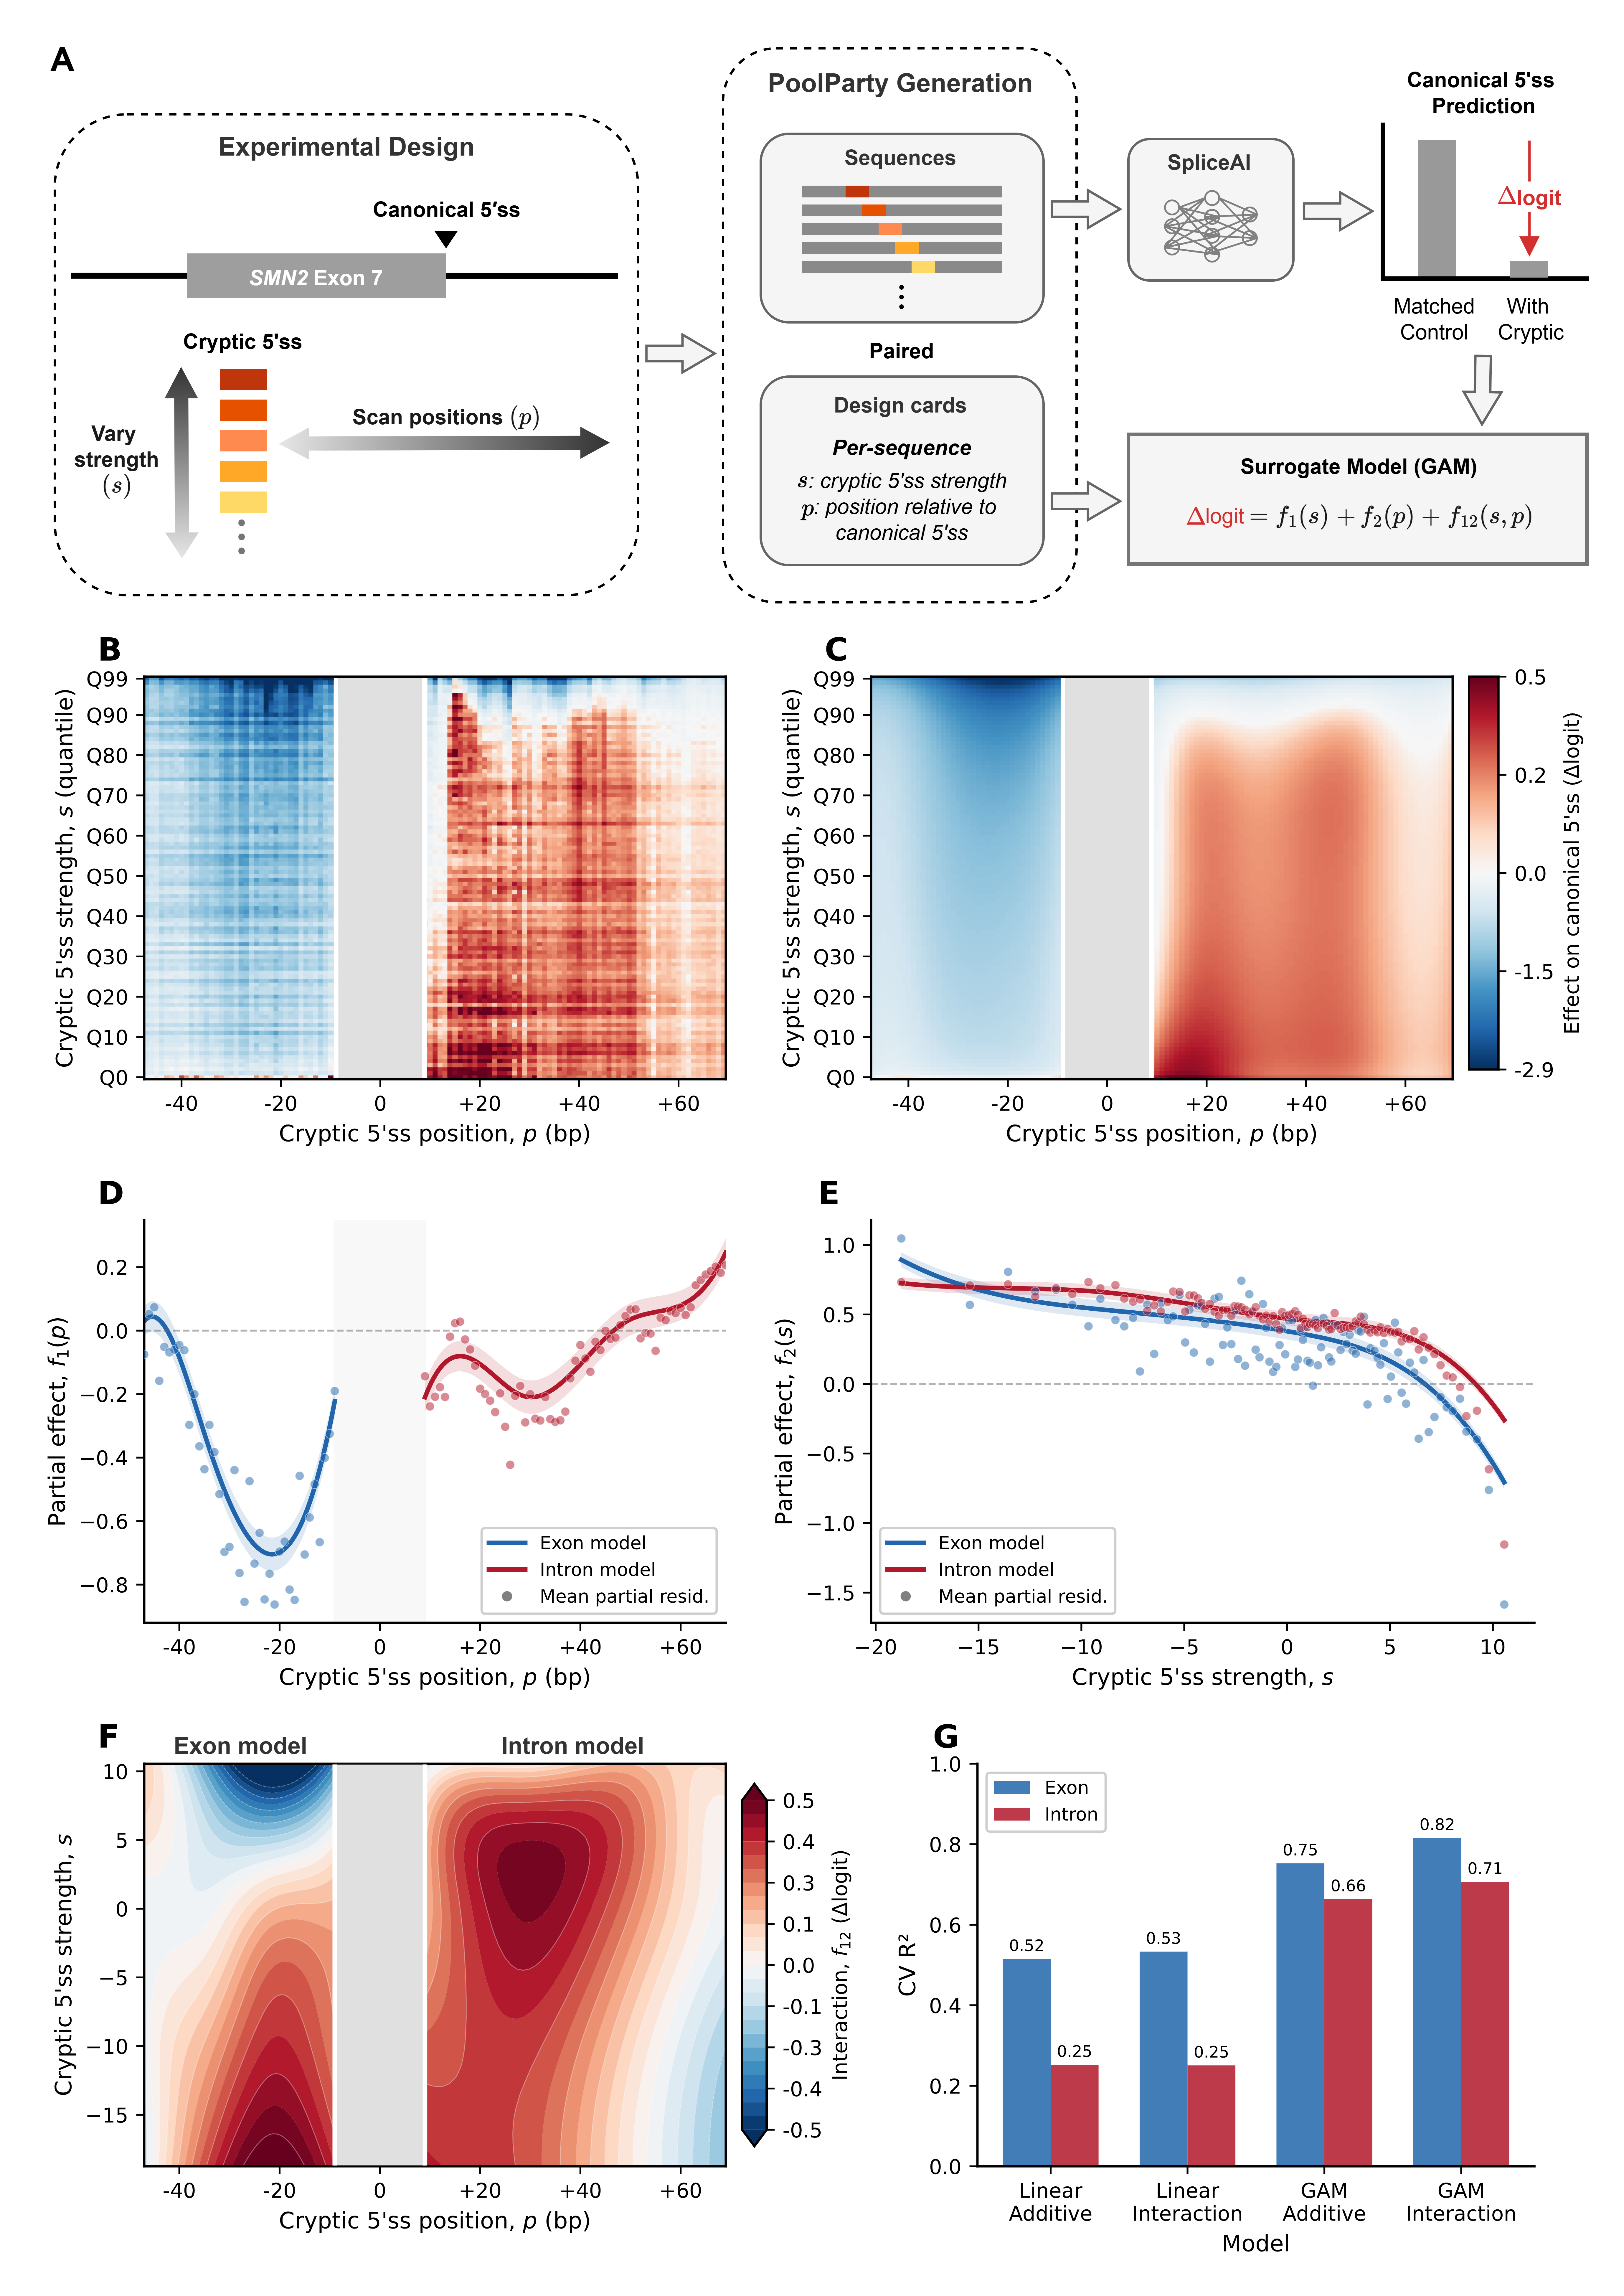
\includegraphics[width=0.85\textwidth]{figure4.png}
\caption{\textbf{Surrogate modeling of SpliceAI predictions using design-card features.}
\textbf{(A)} Experimental design. Cryptic 5$'$ss 9-mers spanning a range of MaxEntScan strengths ($s$) are inserted at positions ($p$) flanking the SMN2 exon~7 canonical donor. Paired library (GT) and control (GA) sequences are generated by PoolParty, and $s$ and $p$ are recorded in design cards. SpliceAI predictions at the canonical donor are summarized as $\Delta$logit and modeled as a function of $s$ and $p$ using a generalized additive model (GAM).
\textbf{(B)} Mean $\Delta$logit across the strength $\times$ position grid ($100 \times 100$; each cell averages 20 distinct 9-mers). The grey band marks the canonical donor region.
\textbf{(C)} GAM interaction model predictions using the same color scale as in B.
\textbf{(D)} Partial dependence of the position term $f_1(p)$, shown separately for exon (blue) and intron (red) models. Shaded regions indicate 95\% confidence intervals; points denote mean partial residuals.
\textbf{(E)} Partial dependence of the strength term $f_2(s)$, with conventions as in D.
\textbf{(F)} Interaction surface $f_{12}(s,p)$ for exon and intron models.
\textbf{(G)} Block cross-validation $R^2$ for linear and GAM models, with and without interaction terms.}
\label{fig:figure4}
\end{figure*}

\subsection{Surrogate modeling of SpliceAI predictions}

In silico libraries designed in the same spirit as MPRAs are increasingly used to probe the regulatory mechanisms learned by genomic deep learning models, treating these models as virtual assays \citep{Avsec2021bpnet, Toneyan2024creme, Seitz2024squid, Nagai2026review}. After scoring these libraries with the model, the relationships between perturbed sequence features and predicted outcomes can be summarized by functions of simpler mathematical form that are intrinsically interpretable, an approach called surrogate modeling. PoolParty streamlines this process through design cards, which record the sequence changes defining each variant and can serve directly as covariates for surrogate models. As a third use case, we apply this approach to characterize the effect of cryptic donor insertion on canonical 5’ss strength as judged by SpliceAI \citep{Jaganathan2019ps}.

Using PoolParty, we designed a library by varying the strength (MaxEntScan) of inserted cryptic donors and their position relative to the canonical 5'ss of SMN2 exon 7 (Methods). The library covered a full grid of 100 positions and 100 strength quantile bins, with design cards automatically recording these parameters for each variant (Fig.~4A). We paired each variant with a matched control and defined the cryptic donor effect as the difference in SpliceAI predictions at the canonical 5'ss between the two. Separate generalized additive models (GAMs) were fit to this quantity for exonic and intronic regions, using only smooth spline terms for strength, position, and their interaction (Fig.~4A).

The GAMs achieved a held-out $R^2$ of 0.82 (exon) and 0.71 (intron), and their response surfaces matched the observed data (Fig.~4B,C). Positional effects showed stronger suppression for exonic than intronic cryptic sites (Fig.~4D), with effects peaking at ~20 bp upstream, consistent with a prior report of preferential depletion of decoy donors proximal to annotated 5'sss on the exonic side \citep{Dawes2022empirical}. In terms of strength effects, stronger cryptic donors drove larger suppression in both models (Fig.~4E). Positional and strength effects also interacted in a non-additive manner, as shown by the interaction surface (Fig.~4F). We compared the GAMs to simpler surrogate alternatives and found that incorporating non-linearity and interaction terms enhanced predictive performance (Fig.~4G).

%%%%%%%%%%%%%%%%%%%%%%%%%%%%%%%%%%%%%%%%%%%%%%%%%%%%%%%%%%%
%%% Above is from manuscript_overleaf_26.03.17/main.tex %%%
%%%%%%%%%%%%%%%%%%%%%%%%%%%%%%%%%%%%%%%%%%%%%%%%%%%%%%%%%%%

\section{Discussion}

We have presented PoolParty, a Python package that replaces the ad hoc scripting commonly used to design oligonucleotide libraries with a declarative, composable, and flexible framework. We demonstrated PoolParty by considering three use cases: library design for a DMS experiment on protein GB1; library design for an MPRA studying transcriptional regulatory grammar; and a surrogate modeling analysis of the effects that cryptic donor sites have on the alternative splicing predictions of SpliceAI. These examples illustrate the flexibility of PoolParty and its applicability to experimental and computational studies.

We wish to highlight the design card that PoolParty returns with each generated sequence. By providing a structured record of how each sequence was constructed, PoolParty facilitates the use of sequence design parameters as covariates in downstream analysis. In the SpliceAI example, the design cards enabled surrogate modeling without any post hoc sequence parsing; we expect this pattern to generalize to the systematic interrogation of other genomic AI models.

PoolParty was designed to address a focused computational problem: provide a lightweight tool for streamlining the design of DNA sequence libraries. Although PoolParty does provide a \texttt{filter} Operation that allows users to remove undesirable sequences from a Pool, it is not intended as a bona fide sequence optimization tool, e.g., for designing synthetic proteins or cis-regulatory elements. Moreover, the current implementation generates sequences one at a time, requiring roughly one millisecond per sequence on a standard laptop. This suffices for typical oligonucleotide libraries but could bottleneck large-scale tasks; a future implementation of batch-mode sequence generation would address this.

We therefore anticipate that PoolParty will substantially ease the design of MPRAs and DMS experiments, as well as other high-throughput functional genomics assays. And as genomic AI models become increasingly accurate, PoolParty will accelerate efforts to gain insight into the molecular mechanisms that underlie the predictions of these models. 

\section{Competing interests}
The authors declare no competing interests. 

\section{Author contributions statement}
Z.L. conceived the project. Z.L. and J.B.K designed the project, wrote the software, performed the analyses, and wrote the manuscript. J.B.K supervised the research. 

\section{Acknowledgments}
This work was supported in part by: NIH grants R01HG011787 (J.B.K, Z.L.). Computational equiptment was supported by NIH grant S10OD028632.

\bibliography{reference}
\end{document}
